
\documentclass[border=10pt]{standalone}
\usepackage{pgfplots}
\pgfplotsset{compat=1.18}
\begin{document}
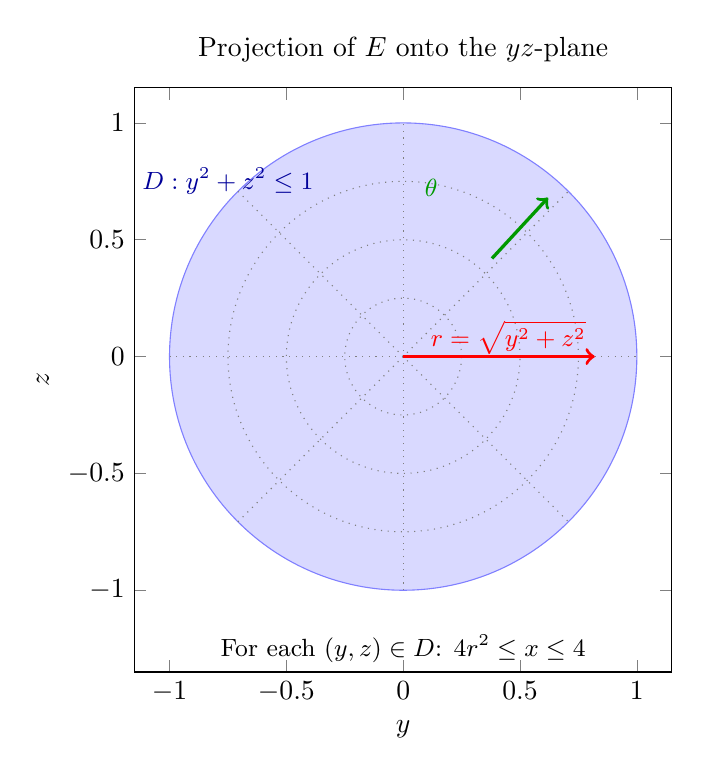
\begin{tikzpicture}
\begin{axis}[
    axis equal image,
    xlabel=$y$, ylabel=$z$,
    xmin=-1.15, xmax=1.15,
    ymin=-1.35, ymax=1.15,
    width=9cm, height=9cm,
    title={Projection of $E$ onto the $yz$-plane},
    clip=false,
]
\fill[blue!15] (axis cs:0,0) circle[radius=1];
\draw[blue!50] (axis cs:0,0) circle[radius=1];
\draw[gray, dotted] (axis cs:0,0) circle[radius=0.25];
\draw[gray, dotted] (axis cs:0,0) circle[radius=0.5];
\draw[gray, dotted] (axis cs:0,0) circle[radius=0.75];
\draw[gray, dotted] (axis cs:-1,0) -- (axis cs:1,0);
\draw[gray, dotted] (axis cs:0,-1) -- (axis cs:0,1);
\draw[gray, dotted] (axis cs:-0.707,-0.707) -- (axis cs:0.707,0.707);
\draw[gray, dotted] (axis cs:-0.707,0.707) -- (axis cs:0.707,-0.707);
\draw[->, red, very thick] (axis cs:0,0) -- (axis cs:0.82,0);
\node[red, font=\small] at (axis cs:0.45,0.08) {$r=\sqrt{y^2+z^2}$};
\draw[->, green!60!black, very thick] (axis cs:0.38,0.42) -- (axis cs:0.62,0.68);
\node[green!60!black, font=\small] at (axis cs:0.12,0.72) {$\theta$};
\node[font=\small] at (axis cs:0,-1.25) {For each $(y,z)\in D$: $4r^2\le x\le 4$};
\node[blue!60!black, font=\small] at (axis cs:-0.75,0.75) {$D:y^2+z^2\le1$};
\end{axis}
\end{tikzpicture}
\end{document}
